\section{Evaluation}

\subsection{Lucene Evaluation}

We begin by quantifying the performance impact of static and dynamic DRAM partitioning under varying budgets. 
For both the M1 and M2 workloads, we collect metrics including total execution time, 
young GC time, mixed GC time. These metrics highlight how each configuration 
responds to increasing memory pressure.

Figures~\ref{fig:m1-exec} and~\ref{fig:m2-exec} summarize the normalized execution time breakdown for both workloads.
Each DRAM setting is shown as a pair of bars: the left bar corresponds to the static TeraHeap (TH) configuration, 
and the right to the dynamic FlexHeap (FH).

Each bar is split into three regions: 
light gray indicates non-GC execution time, 
blue represents young GC time, 
and orange captures mixed GC time.

\begin{figure}[htbp]
  \centering
  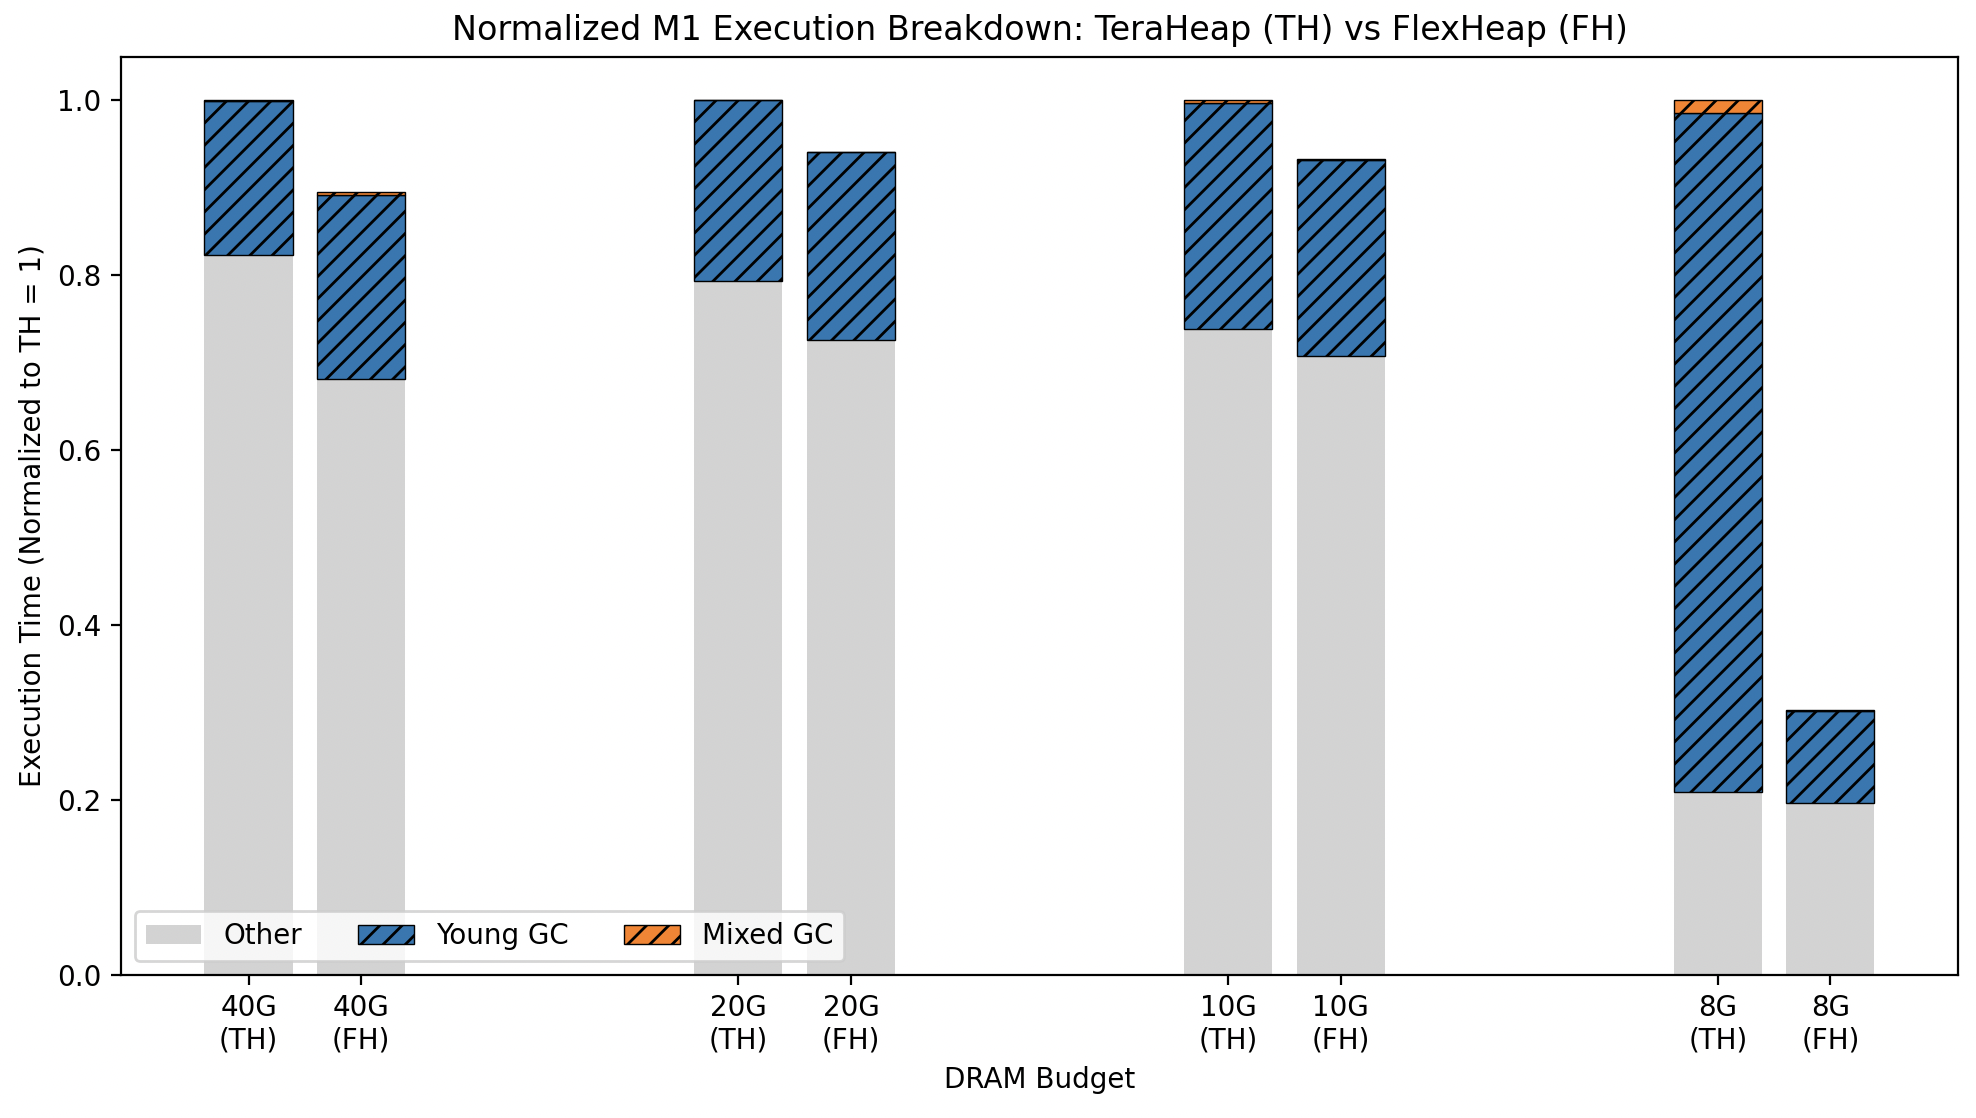
\includegraphics[width=0.95\linewidth]{fig/M1_exec.png}
  \caption{Normalized execution time breakdown for M1 workload.}
  \label{fig:m1-exec}
\end{figure}

\begin{figure}[htbp]
  \centering
  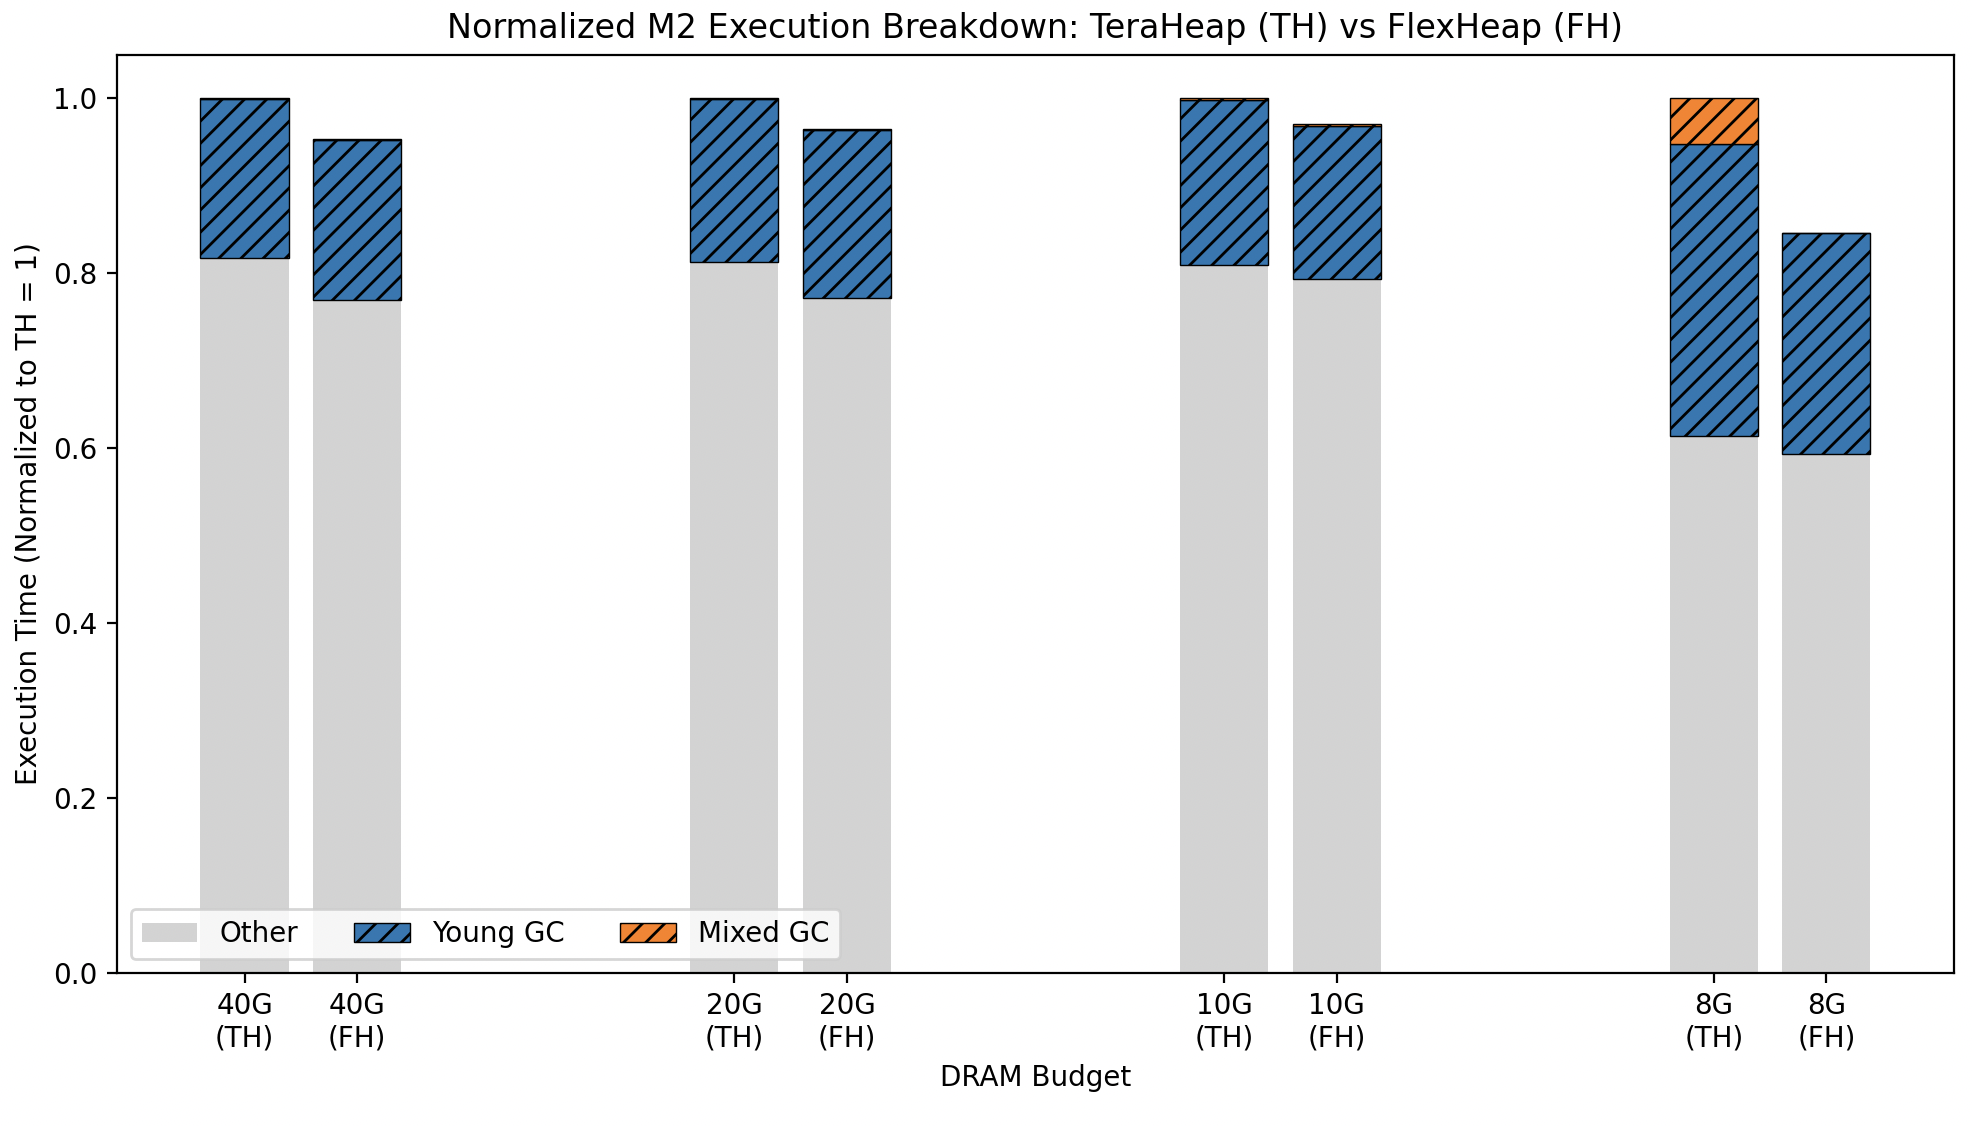
\includegraphics[width=0.95\linewidth]{fig/M2_exec.png}
  \caption{Normalized execution time breakdown for M2 workload.}
  \label{fig:m2-exec}
\end{figure}

In both benchmarks, FlexHeap consistently outperforms TeraHeap, particularly under smaller memory budgets.  
For M1, FlexHeap achieves execution time reductions of 10.4\%, 5.9\%, 6.7\% and 70\% at 40\,G, 20\,G, 10\,G and 8\,G DRAM.
M2 also benefits from FlexHeap, with execution times reduced 
by 4.7\% at 40\,G, 3.5\% at 20\,G, 2.9\% at 10\,G, and 25.4\% at 8\,G. 

FlexHeap also reduces read traffic on the H2 file device.
As shown in Table~\ref{tab:m1-traffic}, FlexHeap lowers read traffic for M1 by 93.6\%, 
91.1\%, and 65.7\% at 20\,G, 10\,G, and 8\,G DRAM, respectively. At 40\,G DRAM, read traffic increases 
by 117.4\%, with also slightly higher GC time but, still reports faster execution due to better tail 
latency (99th percentile latency improves from 1350\,ms to 1327\,ms) and reports higher throughput (Queries Per Second).

For M2, as presented in Table~\ref{tab:m2-traffic}, FlexHeap reduces read traffic consistently across all DRAM configurations by 57.0\% at 40\,G, 
92.2\% at 20\,G, 88.9\% at 10\,G, and 71.5\% at 8\,G while also improving GC and execution time with better latency and higher QPS. 


\begin{table}[h]
\centering
\caption{Read Traffic on H2 file device for M1 workload (in G)}
\label{tab:m1-traffic}
\begin{tabular}{|c|cc|c|}
\hline
% \textbf{DRAM} & \multicolumn{2}{c|}{\textbf{Read Traffic (G)}} & \multicolumn{2}{c|}{\textbf{Write Traffic (G)}} \\
% \textbf{Budget} & TH & FH & TH & FH \\
% \hline
% 40G & 0,938 & 2,039 & 104,075  & 109,4 \\
% 20G & 44,823 & 2,854 & 107,866 & 107,231 \\
% 10G & 287,303 & 25,653 & 108,43 & 109,018 \\
% 8G  & 249,536 & 85,598 & 115,64 & 107,125 \\

\textbf{DRAM} & \multicolumn{2}{c|}{\textbf{Read Traffic(G)}} & \textbf{Reduction} \\
\textbf{Budget} & TH & FH & \textbf(\%)\\
\hline
40G & 0,938 & 2,039 & 117,38 \\
20G & 44,823 & 2,854 & -93,63 \\
10G & 287,303 & 25,653 & -91,07 \\
8G  & 249,536 & 85,598 & 65,7 \\
\hline
\end{tabular}
\end{table}
%
% \begin{table}[t]
%     \centering
%     \caption{Read Traffic on H2 file device for M1 workload (in G)}
%     \label{tab:m1-traffic}
%     \begin{tabular}{lccc}
%         \textbf{Benchmark} & \textbf{TeraHeap (TH)} & \textbf{FlexHeap (FH)} & \textbf{Reduction (\%)} 
%         % \hline
%         40G & 0,938 & 2,039 & 117,38 \\
%         20G & 44,823 & 2,854 & -93,63 \\
%         10G & 287,303 & 25,653 & -91,07 \\
%         8G  & 249,536 & 85,598 & 65,7 \\
%         % \hline
%     \end{tabular}
% \end{table}


\begin{table}[h]
\centering
\caption{Read Traffic on H2 file device for M2 workload (in G)}
\label{tab:m2-traffic}
\begin{tabular}{|c|cc|c|}
\hline
\textbf{DRAM} & \multicolumn{2}{c|}{\textbf{Read Traffic(G)}} & \textbf{Reduction} \\
\textbf{Budget} & TH & FH & \textbf(\%)\\
\hline
40G & 0,679 & 0,292 & -57 \\ 
20G & 11,402 & 0,895 & -92 \\
10G & 109,527 & 12,18 & -89 \\
8G  & 50,936 & 14,538 & -71 \\
\hline
\end{tabular}
\end{table}

% \begin{table}[t]
%     \centering
%     \caption{Read Traffic on H2 file device for M2 workload (in G)}
%     \label{tab:m2-traffic}
%     \begin{tabular}{lccc}
%         % \toprule
%         \textbf{Benchmark} & \textbf{TeraHeap (TH)} & \textbf{FlexHeap (FH)} & \textbf{Reduction (\%)} 
%
%         % \hline
%         % \midrule
%         40G & 0,679 & 0,292 & -57 \\ 
%         20G & 11,402 & 0,895 & -92 \\
%         10G & 109,527 & 12,18 & -89 \\
%         8G  & 50,936 & 14,538 & -71 \\
%         % \hline
%         % \bottomrule
%     \end{tabular}
% \end{table}


Figure~\ref{fig:m2-iow-cpu} provides a visual breakdown of the M2 workload execution under an
8\,G DRAM budget for both TeraHeap and FlexHeap. The top-left subplot shows the TeraHeap run with static DRAM division, 
while the top-right depicts the FlexHeap run. Below each of these, the corresponding I/O wait timelines are shown.

The red line represents the DRAM allocated to the OS page cache, the blue line shows the
amount of used heap (H1) and in the case of TeraHeap, a flat purple line indicates the fixed heap capacity at 4\,GB. 
This unchanging purple line in the TeraHeap plot visually confirms that no heap resizing takes place during the run. 

In the TeraHeap case, in the beginning we observe high GC activity suggesting the that the heap 
capacity is insufficient. This phase also coincides with increased I/O wait times, as presented in the 
iowait plot, indicating that data is being read from the H2 file while the page-cache has limited capacity,
resulting in evictions and increasing read traffic. As execution progresses, the iowait continues to spike,
while the heap gradually grows and then drops, implying that there is unused memory that could be 
assigned to the page-cache to reduce I/O.

In contrast, FlexHeap dynamically shrinks and expands the H1 heap based on workload phases. 
At the beginning of execution, the large I/O wait spikes observed in the TeraHeap run are no longer present, 
as FlexHeap performs heap shrinkages to allocate more DRAM to the page cache. 
The graph also reveals that heap expansions occur within the same phase, 
providing sufficient space to the heap.
This adaptability mitigates I/O bottlenecks but also reduces garbage collection pressure, 
as evidenced by a 63\% reduction in total GC time during the run.
As the benchmark continues, the used heap remains low, suggesting that the page-cache could 
benefit from shrink actions in order to utilize the unused memory. This is evident as the iowait
remains low throughout, compared to the TeraHeap run.


\begin{figure}[htbp]
  \centering
  \begin{tabular}{cc}
    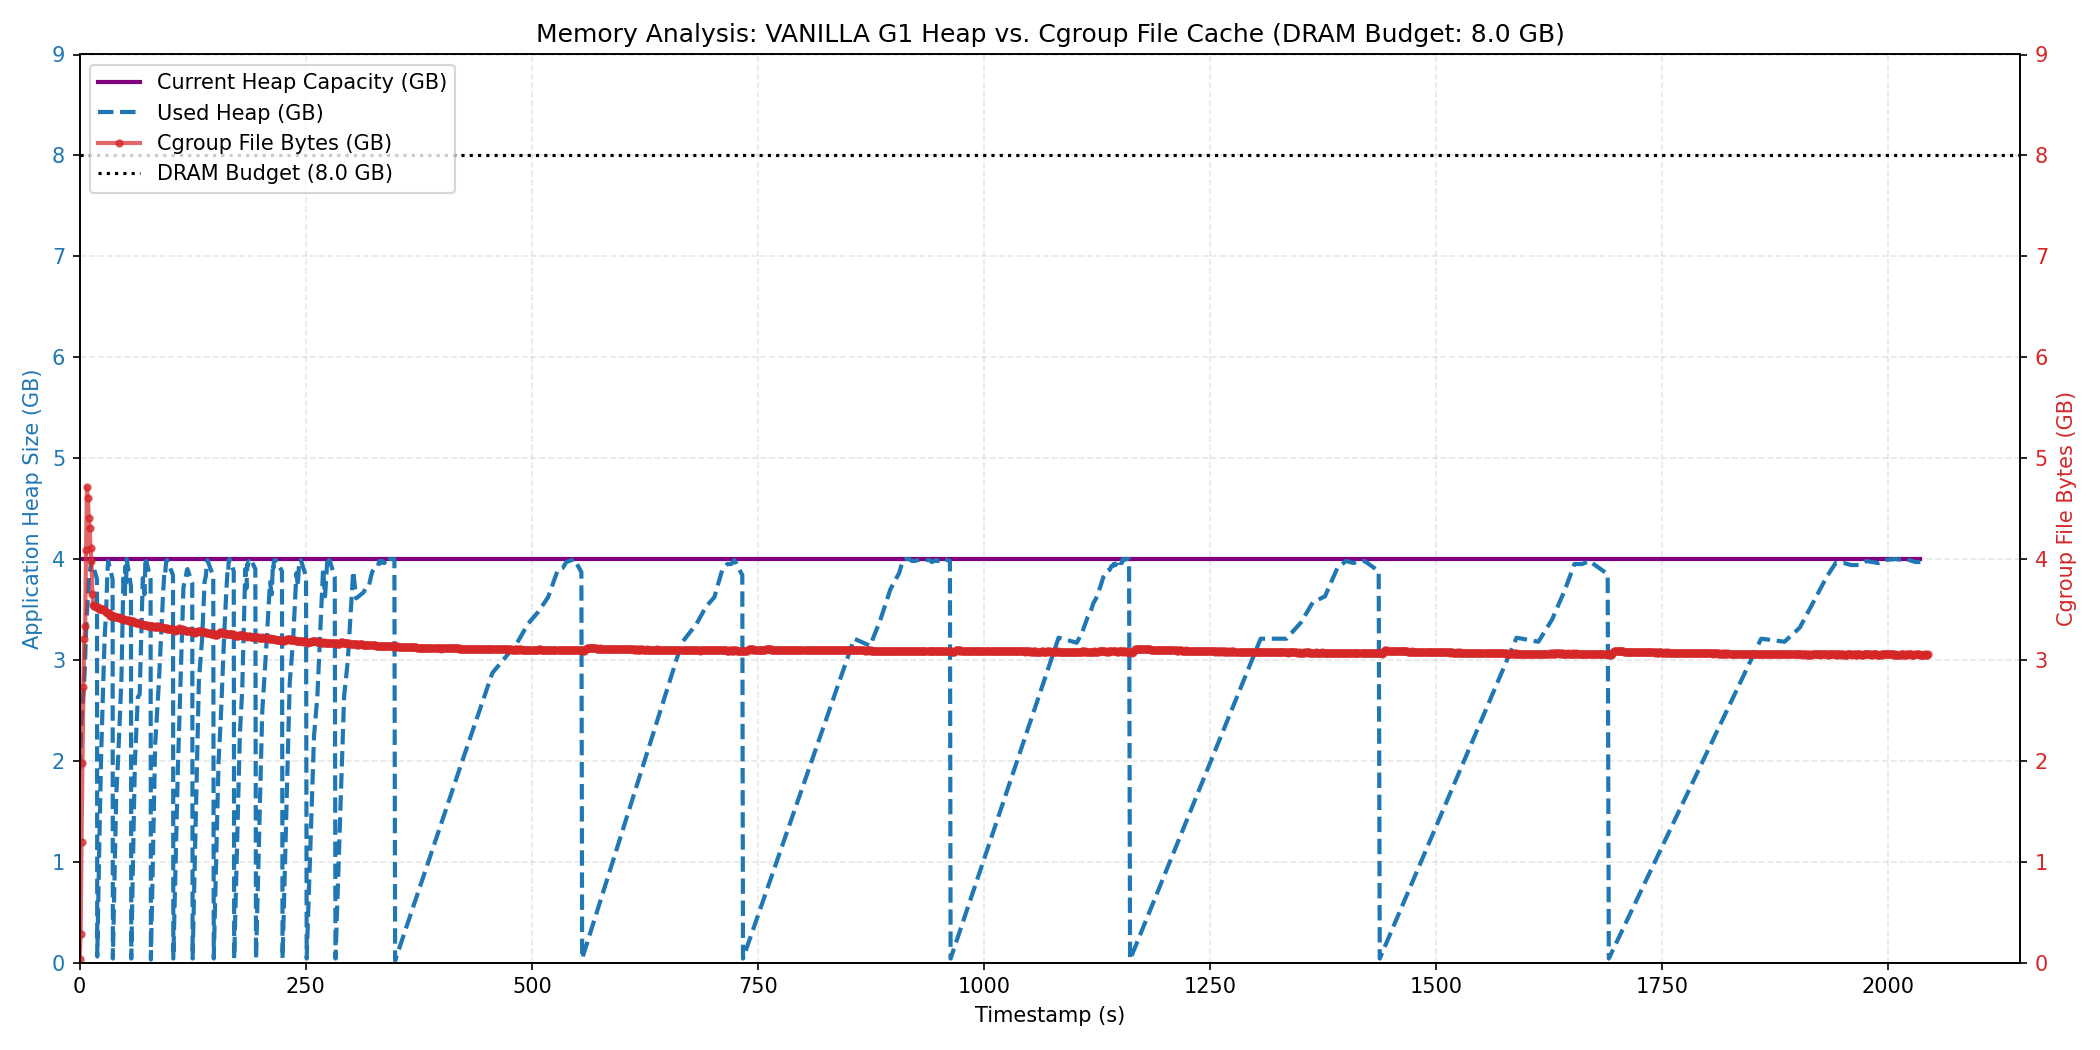
\includegraphics[width=0.48\linewidth]{fig/eval/M2_8DRAM_native.png} &
    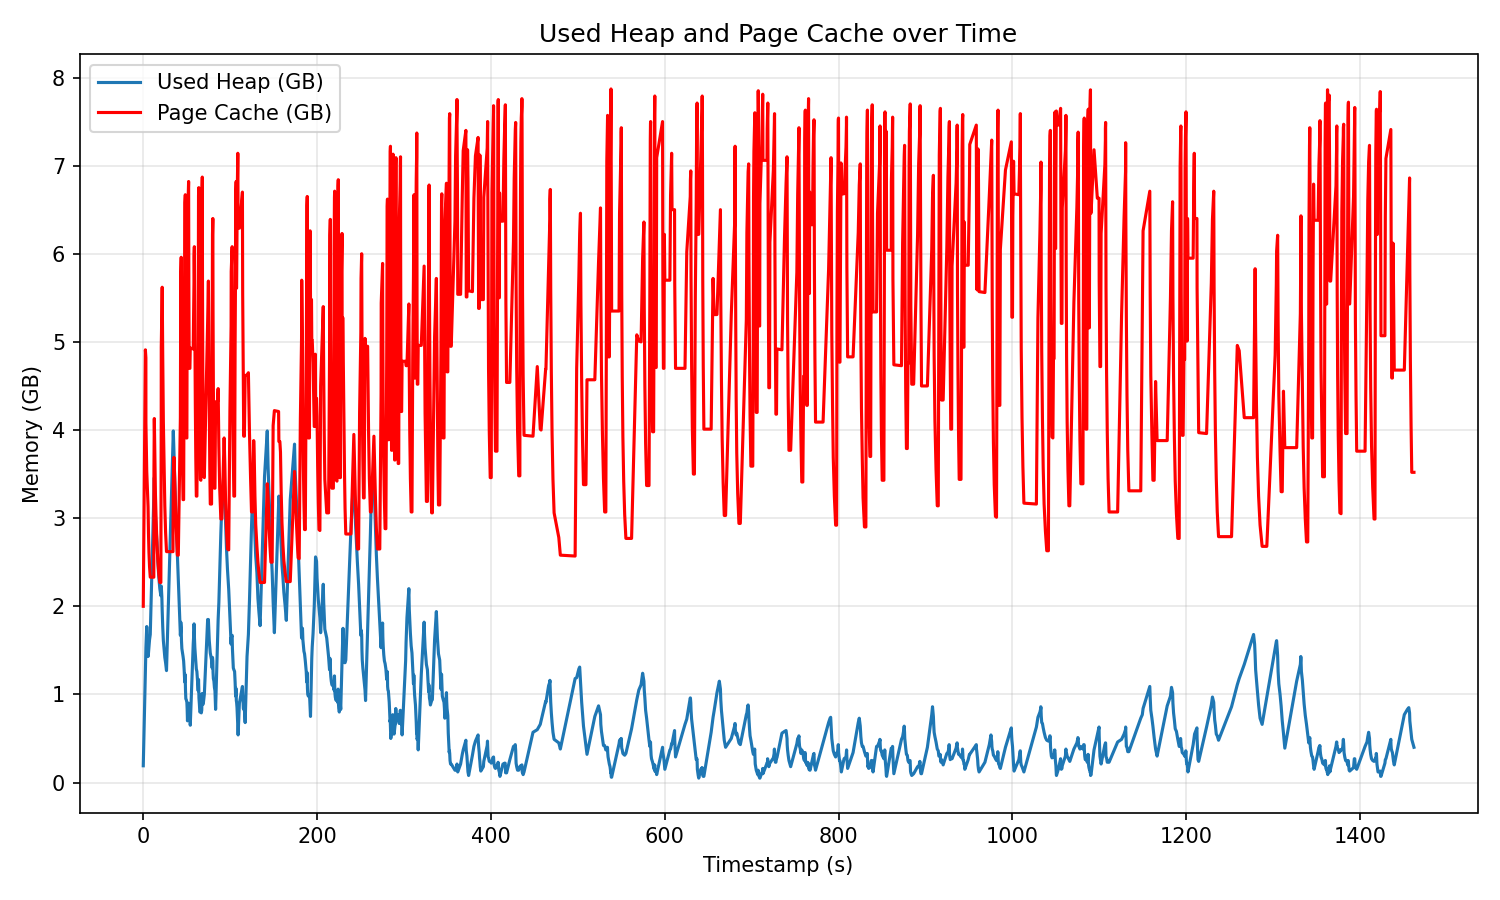
\includegraphics[width=0.48\linewidth]{fig/eval/M2_8DRAM_flex.png} \\
    \small (a) M2 TeraHeap (8\,G DRAM) &
    \small (b) M2 FlexHeap (8\,G DRAM) \\
    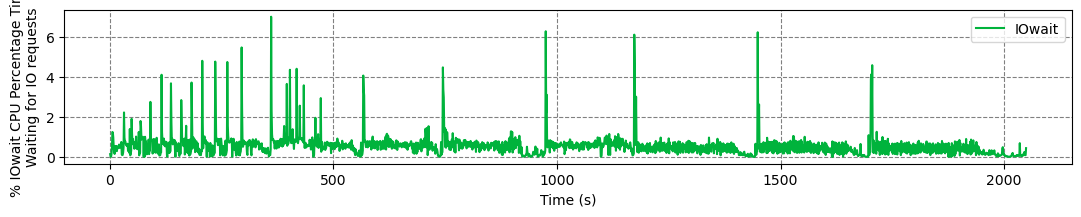
\includegraphics[width=0.48\linewidth]{fig/eval/iow_cpu_native_8DRAM_M2.png} &
    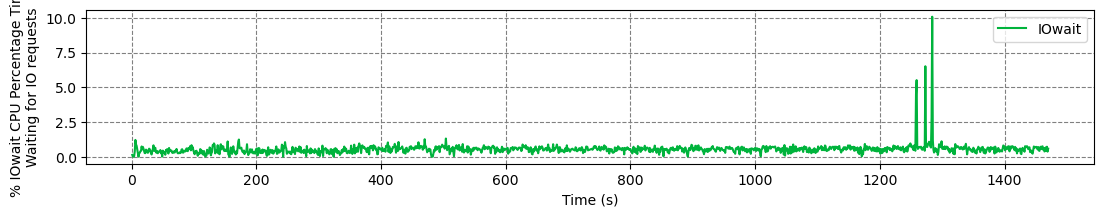
\includegraphics[width=0.48\linewidth]{fig/eval/iow_cpu_flex_8DRAM_M2.png} \\
    \small (c) iowait (TeraHeap) &
    \small (d) iowait (FlexHeap) \\
  \end{tabular}
  \caption{Comparison of CPU and I/O behavior for M2 workload under 8\,G DRAM using TeraHeap (native) and FlexHeap.}
  \label{fig:m2-iow-cpu}
\end{figure}


\vspace{1em}


\subsection{Evaluation on Spark Benchmarks}

\begin{figure}[t]
    \centering
    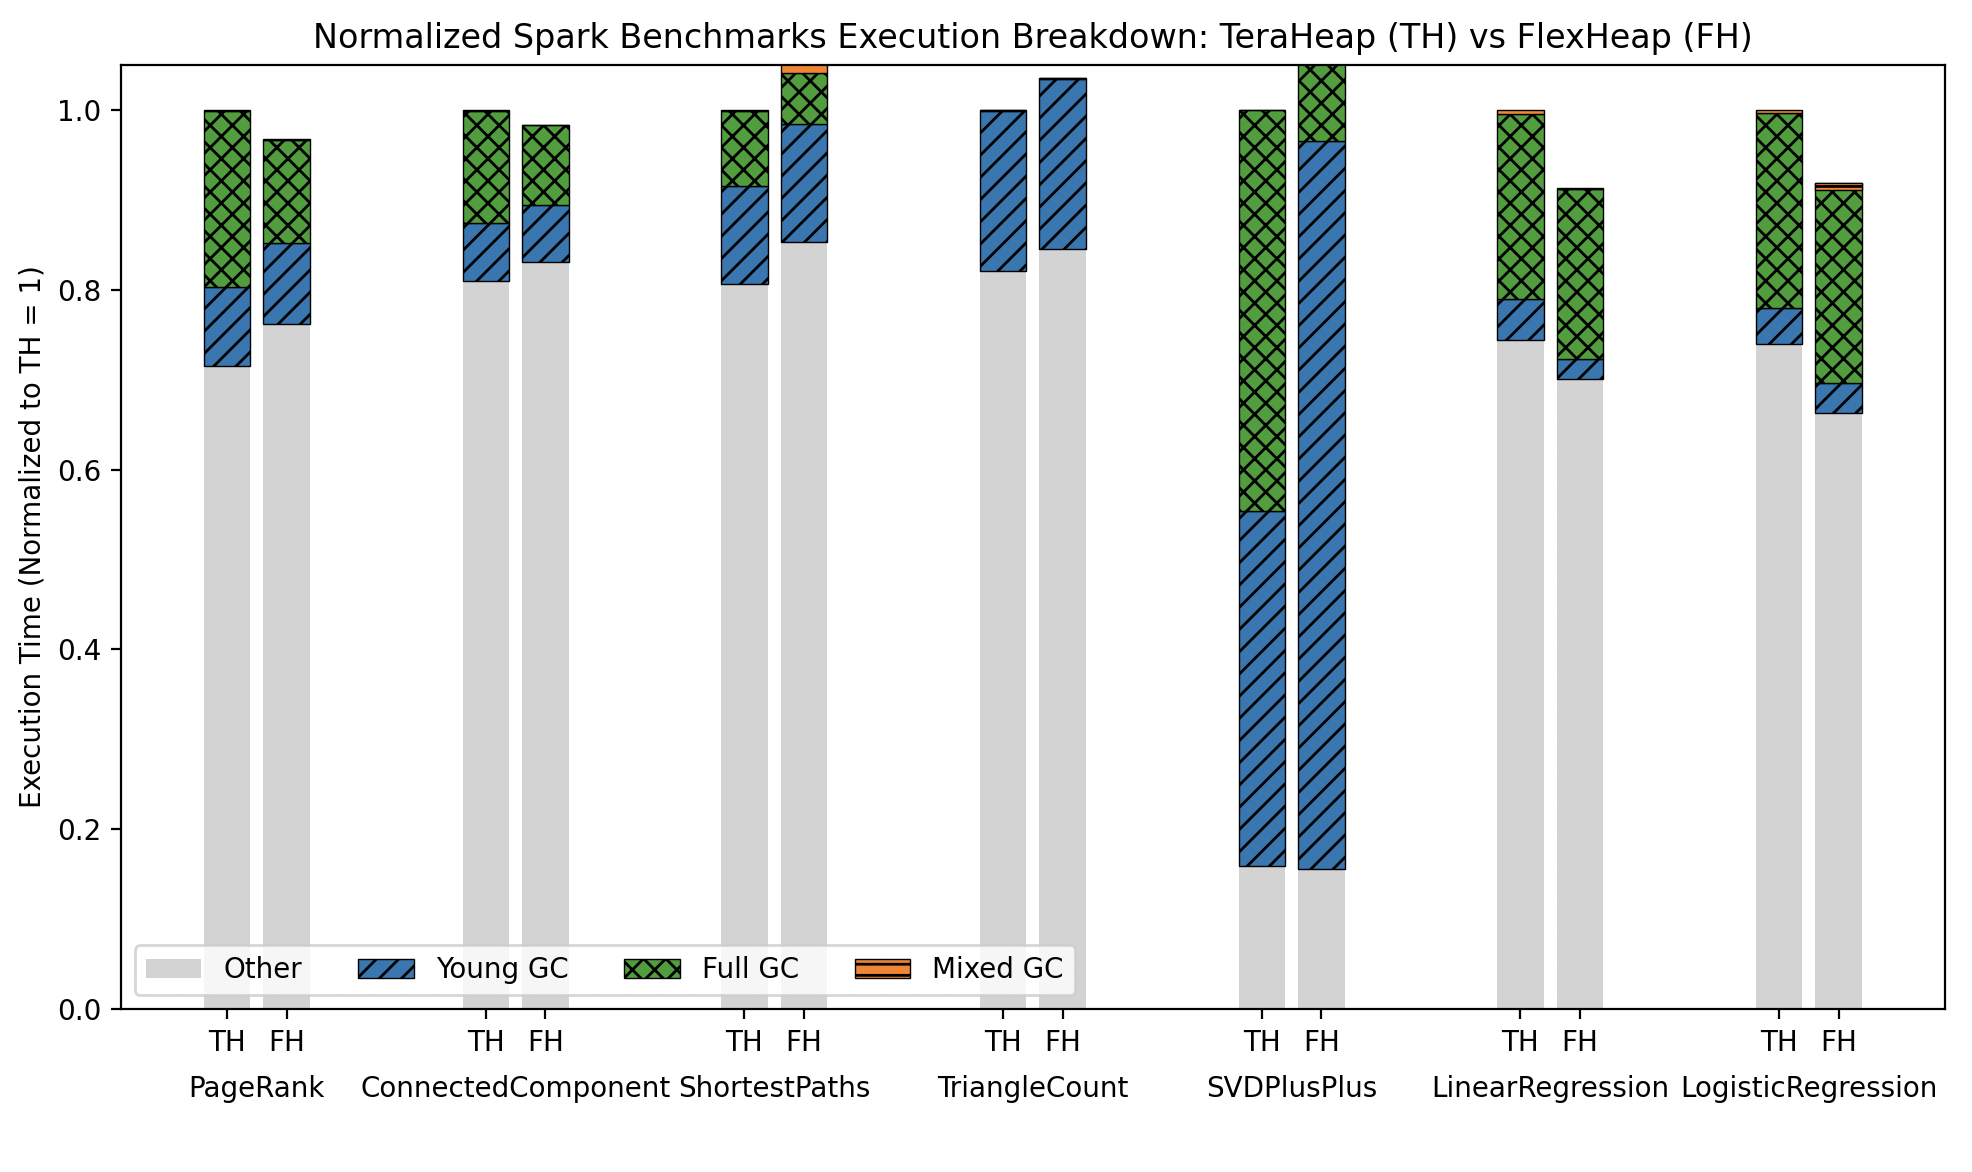
\includegraphics[width=\linewidth]{fig/spark_benchmarks.png}
    \caption{Normalized Spark Benchmarks Execution Breakdown: TeraHeap (TH) vs FlexHeap (FH).}
    \label{fig:spark-eval}
\end{figure}

To evaluate FlexHeap, on Spark,  we run a diverse suite of workloads and compare its performance against TeraHeap. 
Figure~\ref{fig:spark-eval} presents a normalized execution time breakdown across seven Spark benchmarks. 
FlexHeap improves overall execution time in 4 out of 7 workloads \textit{PageRank}, \textit{ConnectedComponent},
\textit{ShortestPaths}, and \textit{LogisticRegression} where it also reduces total garbage collection (GC) time and read traffic, 
on the device that contains the H2 file.

In contrast, benchmarks like \textit{SVDPlusPlus}, \textit{LinearRegression}, and \textit{TriangleCount} report worse execution time compared to TeraHeap.
We analyze these cases in more detail in the following subsections to understand the underlying factors affecting FlexHeap’s effectiveness.

\begin{table}[h]
\centering
\caption{H2 File Device Read Traffic (in G) for Spark Benchmarks}
\label{tab:spark-h2-traffic}
\begin{tabular}{|c|cc|c|}
\hline
\textbf{DRAM} & \multicolumn{2}{c|}{\textbf{Read Traffic(G)}} & \textbf{Reduction} \\
\textbf{Budget} & TH & FH & \textbf(\%)\\
\hline
        PageRank              & 420,57  & 377,01 & -10,36 \\
        ConnectedComponent    & 526,9  & 414,61  & -21,31 \\
        ShortestPaths         & 225,9  & 219,99 & -2,62 \\
        TriangleCount         & 28,56  & 26,81  & -6,11 \\
        SVDPlusPlus           & 261,56  & 349,16 & +33,49 \\
        LinearRegression      & 1584,87  & 1296,74 & -18,14 \\
        LogisticRegression    & 1618,42 & 1157,82 & -28,46 \\
\hline
\end{tabular}
\end{table}


Table~\ref{tab:spark-h2-traffic} reports the total read traffic to the H2 file device for each Spark benchmark under
TeraHeap (TH) and FlexHeap (FH). FlexHeap consistently reduces read traffic in 6 out of the 7 benchmarks,
demonstrating improved interaction with the OS page cache. The reductions range from 2.6\% in \textit{ShortestPaths}
to 28.5\% in \textit{LogisticRegression}, with an average reduction of approximately 14.5\% across these workloads.
The only exception is \textit{SVDPlusPlus}, where read traffic increases by 33.5\%. 

The only exception is \textit{SVDPlusPlus}, where FlexHeap incurs higher read traffic than TeraHeap. 

